\begin{anexosenv}

\partanexos

% Texto do primeiro anexo.

\chapter{\nmu Figuras}
\label{anexos}

% \begin{figure}[h]
%   \centering
% 	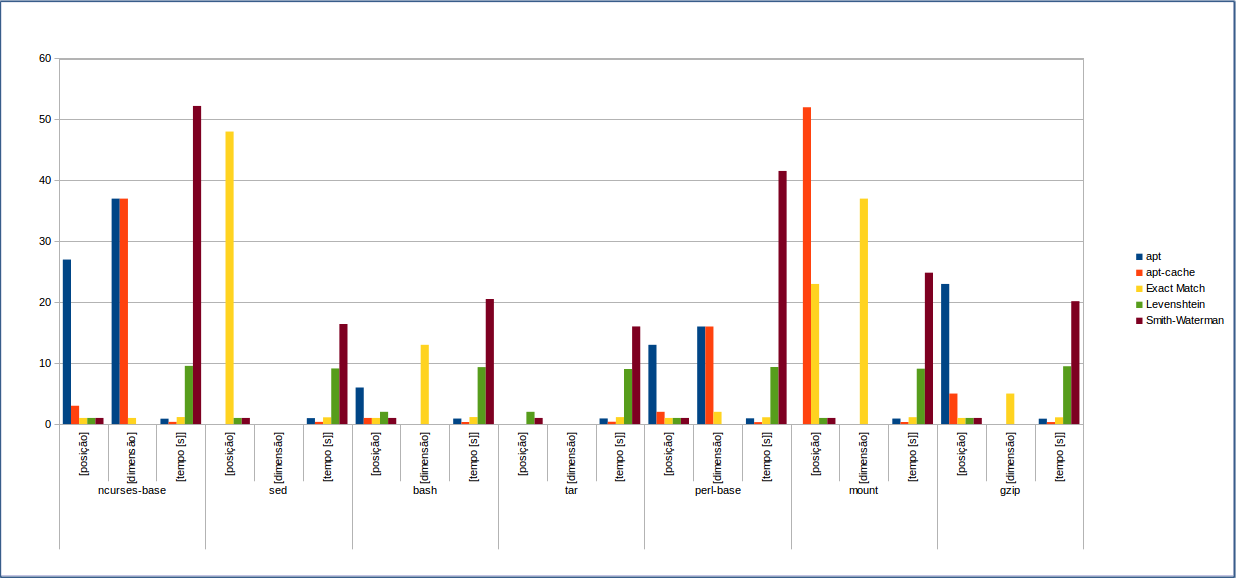
\includegraphics[width=0.7\textheight,angle=90]{figuras/grafico}
%   \caption{Amostra de comparação dos resultados}
%   \label{fig:figuras_grafico}
% \end{figure}
% \cleardoublepage

\begin{figure}[h]
  \centering
	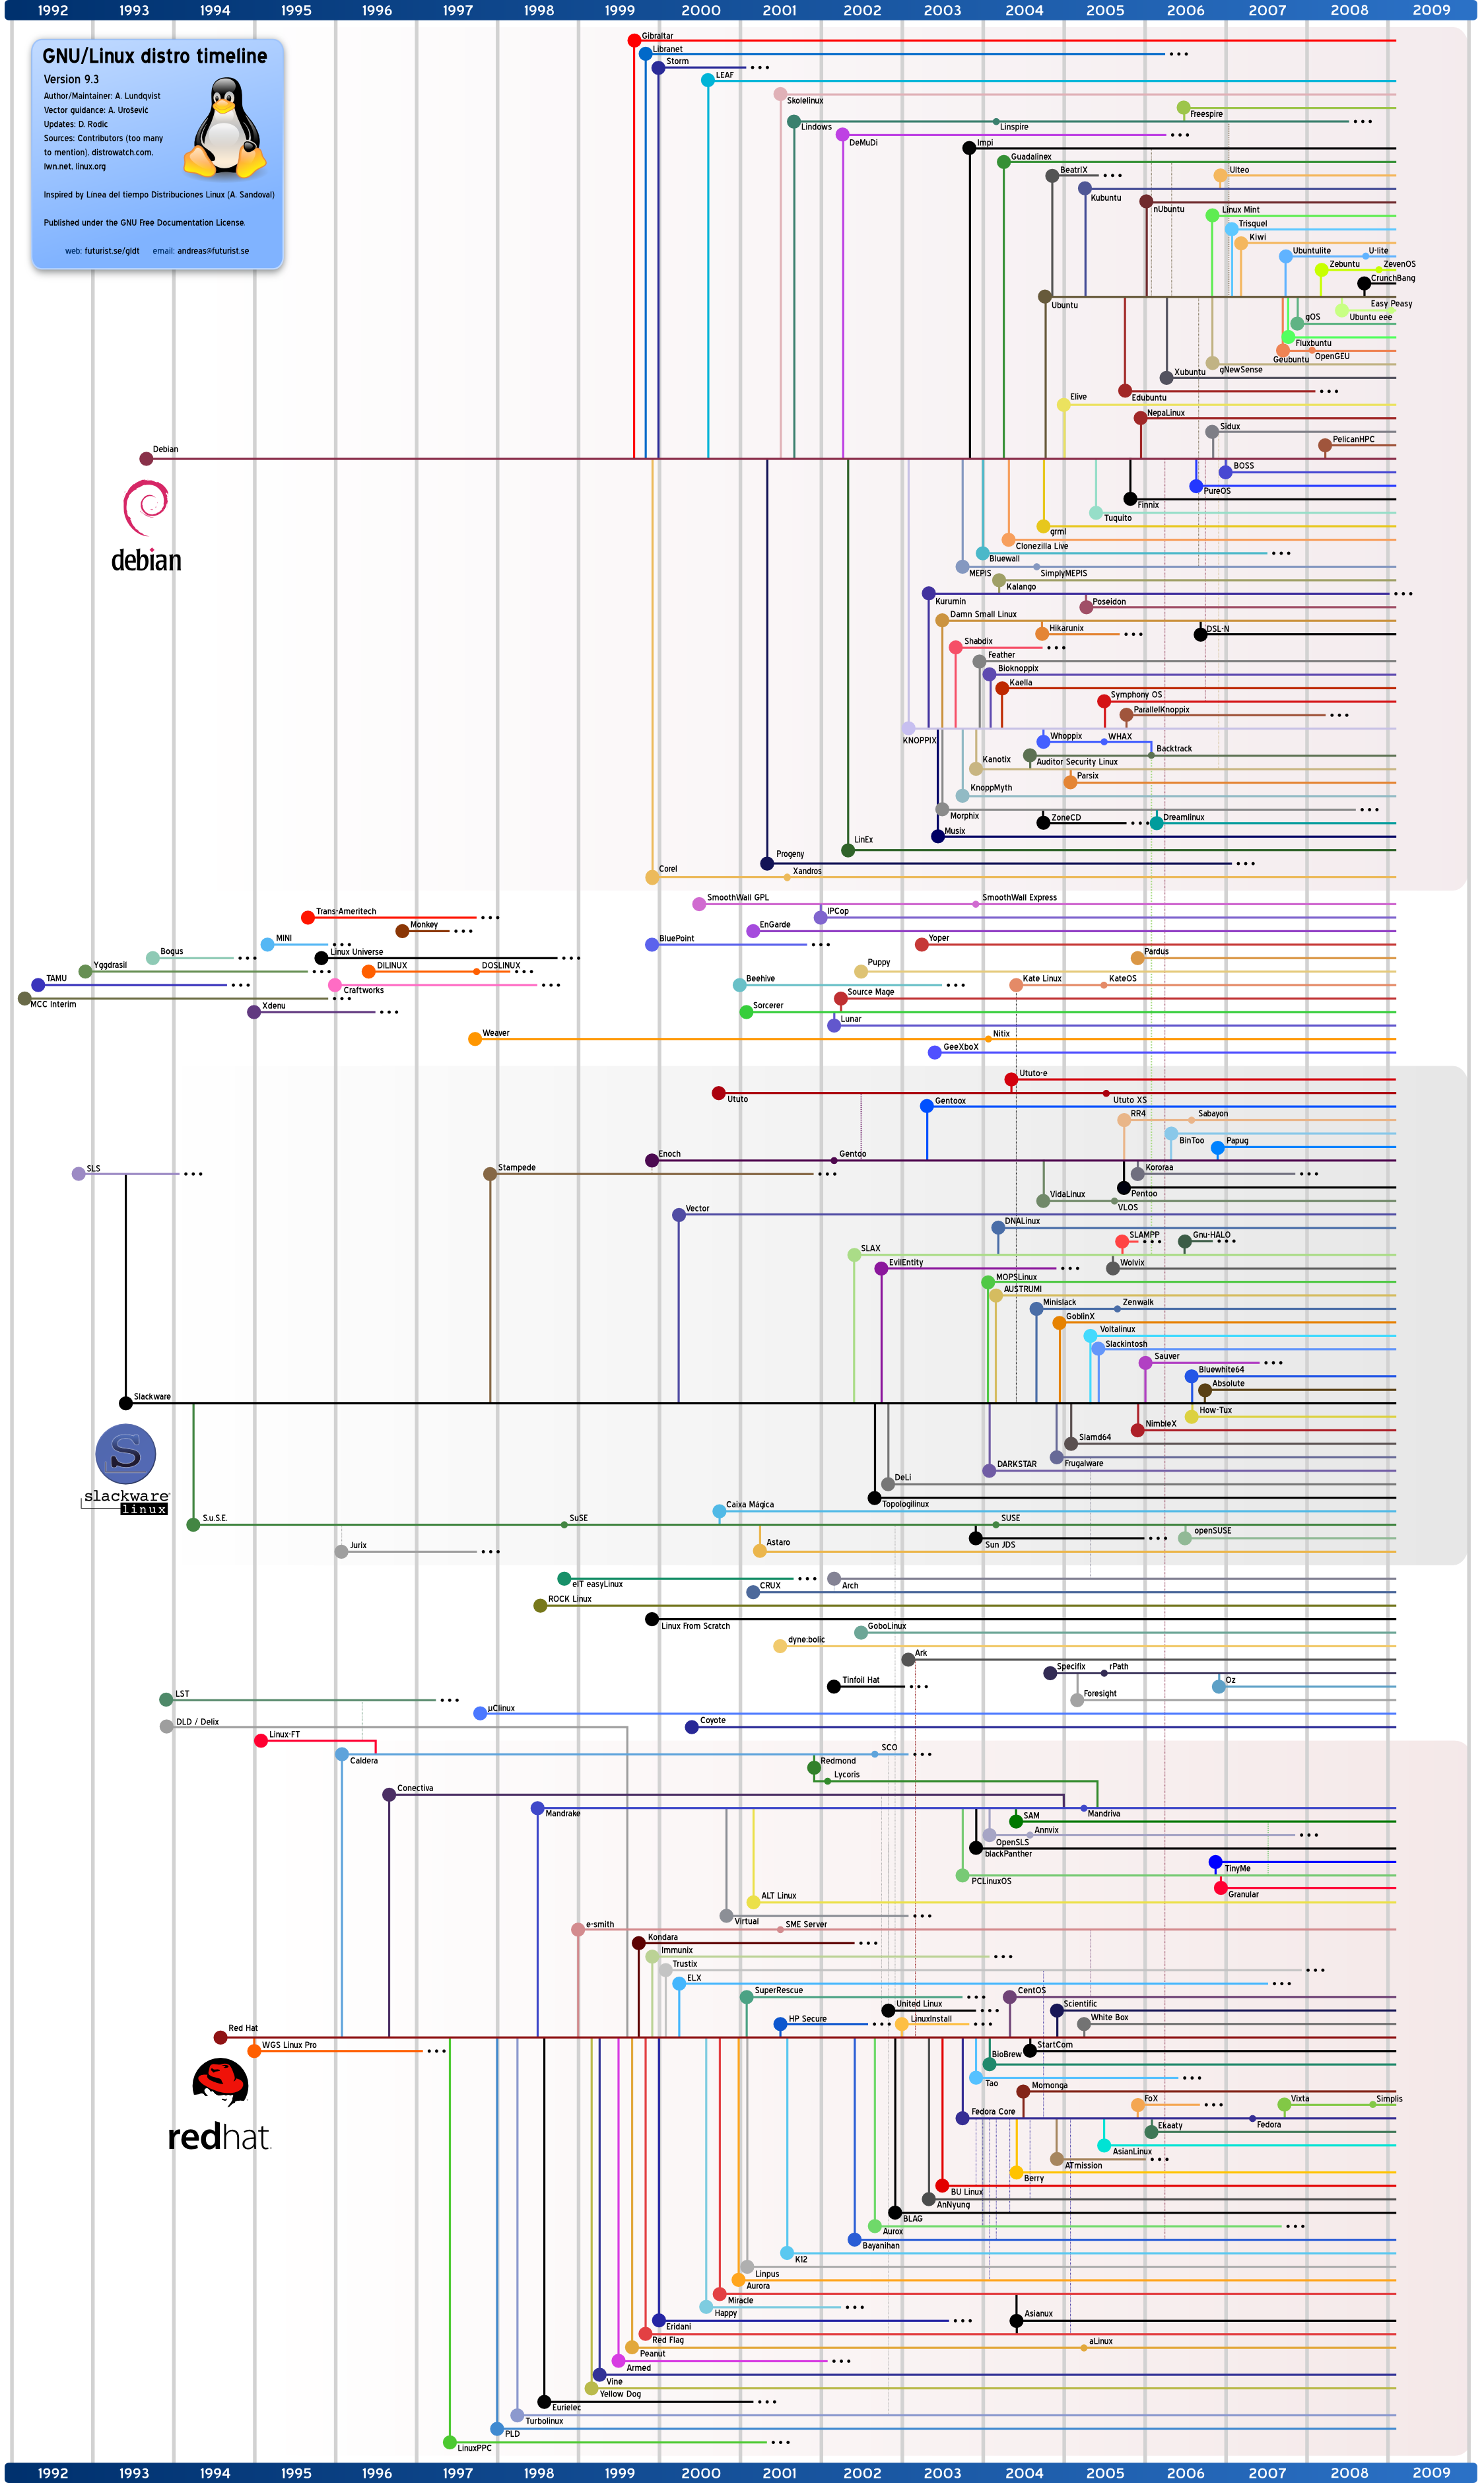
\includegraphics[width=0.75\textwidth]{figuras/linux-timeline-heranca}
  \caption[Heranças de algumas das distribuições Linux existentes hoje]{Heranças de algumas das distribuições Linux existentes hoje\protect\footnotemark.}
  \label{fig:figuras_linux_timeline_heranca}
\end{figure}
\footnotetext{\label{note:figuras_linux_timeline_heranca}\textbf{Fote:} \href{http://www.linux-es.org/files/distribuciones_en_el_tiempo.png}{www.linux-es.org}}

A \autoref{fig:figuras_linux_timeline_heranca} apresenta uma  visualização de algumas das ramificações que surgiram cronologicamente nas distribuições Linux, dando um foco para  as três distribuições comentadas neste estudo: \textit{Debian, Slackware} e \textit{Red Hat}. A linha na horizontal indica a \textit{timeline} da distribuição. As reticencias ao final da linha indicam que a distribuição foi descontinuada. As linhas na vertical podem indicar uma ramificação (nova distribuição criada a partir de uma antiga) ou a fusão de distribuições. Linhas na horizontal contendo um circulo no meio do tracejado indicam que alguma distribuição alterou o seu  nome (como foi o caso do S.u.S.E para SuSE no ano de 1998). Mesmo que de dificil visualização do nome das distribuições na imagem, o objetivo dela no trabalho é contextualizar a influencia que as distribuições \textit{Debian, Slackware} e \textit{Red Hat} tem entre diversas distribuições e que novas funcionalidades nelas serão eventualmente adotadas nas suas herdeiras, aumentando a propagação de funcionalidades. Assim, uma nova funcionalidade no \textit{Debian} certamente seria adotada na distribuição \textit{Ubuntu} e suas ramificações, porém novas funcionalidades no \textit{Ubuntu} demoram a serem copiadas para o \textit{Debian}, quando são. Uma adaptação da imagem \textit{Linea del tiempo Distribuciones Linux}, a imagem pode ser melhor vizualizada em \url{http://www.linux-es.org/files/distribuciones_en_el_tiempo.png}.

% Texto do segundo anexo.

\end{anexosenv}

